
\section{平坦性蕴含欧拉示性数恒常}

我们来实现 \S24.0.1 中许诺过的\trFlatness{}的一个重要推论。将会看到，这一结果为许多我们在还不知道平坦性时就该问起的问题给出答案与实例。

\textbf{24.7.1. 重要定理（欧拉示性数在平坦\trFamily{}中恒常）。}\ ——\ \emph{设 $\pi\colon X\to Y$ 是局部\trNoether{}\trScheme{}之间的一个\trProjective{}\trMorphism，$\mathscr{F}$ 是 $X$ 上的一个\trCoherentSheaf，在 $Y$ 上\trFlat。则 $\chi(X_q,\mathscr{F}|_{X_q})=\sum_{i\ge 0}(-1)^i h^i(X_q,\mathscr{F}|_{X_q})$ 是 $q\in Y$ 的\trLocallyConstant{}函数（其中 $X_q=\pi^{-1}(q)$）。}

这是「\trCohomology{}在平坦\trFamily{}中表现良好」的第一个征兆。（我们很快将看到第二个征兆：\mbox{\trSemicontinuity{}定理~25.1.1}。\mbox{定理~24.7.1} 的另一个证明——它把结果推广到\trProper{}情形——将在 \S25.2.5 中给出。）诸\trNoether{}假设的用途，在于保证 $\pi_\ast\mathscr{F}(m)$ 是\trCoherentSheaf。

\mbox{定理~24.7.1} 给出了平坦性的一个必要条件。它的逆命题（给出充分条件）见\mbox{练习~24.7.C}。

\emph{证明。}\quad 我们先作三个快速的化归。（i）这个问题在靶 $Y$ 上局部，故可化归到 $Y$ 仿射的情形，比如说 $Y=\Spec B$，于是 $\pi$ 可通过某个\trClosedEmbedding{} $X\hookrightarrow\mathbb{P}^n_B$（$n$ 为某个数）分解。（ii）把 $\mathscr{F}$ 视为 $\mathbb{P}^n_B$ 上的\trSheaf，便可化归到 $X=\mathbb{P}^n_B$ 的情形。（iii）可化归为证明：对 $m\gg 0$，$h^0(X_q,\mathscr{F}(m)|_{X_q})$ 是 $q\in Y$ 的\trLocallyConstant{}函数，并且当 $i>0$ 时 $h^i(X_q,\mathscr{F}(m)|_{X_q})=0$。（由\trSerre{}消失，当 $i>0$ 且 $m\gg 0$ 时确有 $h^i(X_q,\mathscr{F}(m)|_{X_q})=0$，但先验地每个 $q$ 可各有不同的 $m$，而我们需要 $m$ 不依赖于 $q$。）

取 $m\gg 0$ 并用 $\OO(m)$ 扭转，使得 $\mathscr{F}$ 的高阶\trCohomology{} $\mathrm{H}^{i>0}(X,\mathscr{F}(m))$ 全部消失（由\trSerre{}消失，\mbox{定理~18.1.3}~(ii)）。现在考虑 $\mathscr{F}(m)$ 的\trCech\trComplexN{} $\mathscr{C}^{\bullet}$。注意：由于 $\mathscr{F}$ \trFlat，\trCech\trComplexN{} $\mathscr{C}^{\bullet}$ 的所有项都是平坦的。（你看出缘由了吗？）既然所有高阶\trCohomology{}群（\trHigherPushforward）都消失，$\mathscr{C}^{\bullet}$ 除首项外正合，而首项处的\trCohomology{}是 $\Gamma(\pi_\ast\mathscr{F}(m))$。我们把\trModule{} $\Gamma(\pi_\ast\mathscr{F}(m))$ 添到复形的最前端，它便再次正合：
\[
\tag{24.7.1.1}\label{eq:flat-cech-resolution}
0 \longrightarrow \Gamma(\pi_\ast\mathscr{F}(m)) \longrightarrow \mathscr{C}^1 \longrightarrow \mathscr{C}^2 \longrightarrow \cdots \longrightarrow \mathscr{C}^{n+1} \longrightarrow 0.
\]
（这种把一个\trModule{}「接上去」的把戏我们以前也干过，例如 \eqref{eq:extended-cech-complex}。）于是，由练习~24.2.G，我们有一条除首项外诸项皆平坦的正合列，故首项也是平坦的。于是 $\pi_\ast\mathscr{F}(m)$ 是 $Y$ 上一个平坦的\trCoherentSheaf，从而是\trLocallyFree{}的（\mbox{推论~24.3.7}），从而具有\trLocallyConstant{}的\trRank。

设 $q\in Y$。我们想证明\trHilbert{}函数 $h_{\mathscr{F}|_{X_q}}(m)$ 是 $q$ 的\trLocallyConstant{}函数。为计算 $h_{\mathscr{F}|_{X_q}}(m)$，我们把\trCech{}分解与 $\kappa(q)$ 作张量，再取\trCohomology。\trCech{}分解加上前端所接的 $\Gamma(\pi_\ast\mathscr{F}(m))$——即 \eqref{eq:flat-cech-resolution}——是平坦\trModule{}的正合列，因而与 $\kappa(q)$ 作张量后仍保持正合（\mbox{练习~24.2.F}）。于是
\[
\Gamma(\pi_\ast\mathscr{F}(m))\otimes\kappa(q)\cong\Gamma(\pi_\ast\mathscr{F}(m)|_q),
\]
所以\trHilbert{}函数 $h_{\mathscr{F}|_{X_q}}(m)$ 就是某个\trLocallyFreeSheaf{}在 $q$ 处的\trRank，而这乃是 $q\in Y$ 的\trLocallyConstant{}函数。\hfill$\square$

现在我们来给出\mbox{定理~24.7.1} 的几个有用得离谱的推论。

\textbf{24.7.2. \trhCorollary。}\ ——\ \emph{采用与\mbox{定理~24.7.1} 相同的假设与记号。则 $\mathscr{F}|_{X_q}$ 的\trHilbertPolynomial{}作为 $q\in Y$ 的函数是\trLocallyConstant{}的。}

\textbf{24.7.A.（关键练习）}\quad 设 $X\to Y$ 是\trProjective{}\trFlat{}\trMorphism，其中 $Y$ \trConnected。证明：$q\in Y$ 的下列函数都是常数：（a）\trFiber{}的\trDegree；（b）\trFiber{}的\trDimension；（c）\trFiber{}的\trArithmeticGenus。

\textbf{24.7.B.（练习）}\quad 用 \S24.3.9 与\mbox{练习~24.7.A}(a)，给出\mbox{练习~16.3.D}(a)（「从无\trEmbeddedPoint{}的\trCurve{}到\trIrreducible\trRegular\trCurve{}的\trFinite\trMorphism{}具有常值的\trDegree」）的另一个解法。

\textbf{24.7.C.（不重要练习（\mbox{定理~24.7.1} 的逆命题））}\quad （这个练习我们不会用在任何地方。）
（a）设 $A$ 是\trRing，$S_\bullet$ 是一个在 $A$ 上平坦的有限生成 $A$-\trAlgebra。证明 $\Proj S_\bullet$ 在 $A$ 上\trFlat。
（b）设 $\pi\colon X\to Y$ 是局部\trNoether{}\trScheme{}之间的一个\trProjective{}\trMorphism（一如既往，这包括 $X$ 上一个\trInvertibleSheaf{} $\OO_X(1)$ 的数据），使得对某个 $m_0$ 及一切 $m\ge m_0$，$\pi_\ast\OO_X(m)$ 都是\trLocallyFree{}的。证明 $\pi$ \trFlat。提示：把 $X$ 描述为
\[
\Proj\left(\OO_Y\oplus\Bigl(\bigoplus_{m\ge m_0}\pi_\ast\OO_X(m)\Bigr)\right).
\]
（c）更一般地，设 $\pi\colon X\to Y$ 是局部\trNoether{}\trScheme{}之间的一个\trProjective{}\trMorphism，$\mathscr{F}$ 是 $X$ 上的一个\trCoherentSheaf，使得对某个 $m_0$ 及一切 $m\ge m_0$，$\pi_\ast\mathscr{F}(m)$ 都是\trLocallyFree{}的。证明 $\mathscr{F}$ 在 $Y$ 上\trFlat。
（d）设 $\pi\colon X\to Y$ 是局部\trNoether{}\trScheme{}之间的一个\trProjective{}\trMorphism，$\mathscr{F}$ 是 $X$ 上的一个\trCoherentSheaf，使得 $\mathscr{F}|_{X_q}$ 的\trHilbertPolynomial{}是 $q\in Y$ 的\trLocallyConstant{}函数。若 $Y$ \trReduced，证明 $\mathscr{F}$ 必在 $Y$ 上\trFlat。（提示：\mbox{练习~14.3.K} 表明，在特别好的情形中，常\trRank{}蕴含\trLocallyFree{}性。）

\mbox{推论~24.7.2} 的另一个推论，则惊人地有用。

\textbf{24.7.3. \trhCorollary。}\ ——\ \emph{平坦\trProjective{}\trCurve{}\trFamily{} $X$ 上的\trInvertibleSheaf{} $\mathscr{L}$，在诸\trFiber{}上具有\trLocallyConstant{}的\trDegree。}

（回想：\trProjective{}\trCurve{}上\trLineBundle{}之\trDegree{}的定义，不需要对\trCurve{}附加诸如\trRegularity{}之类的假设；见 \eqref{eq:degree-coherent-sheaf}。）

\emph{证明。}\quad 平坦\trCurve{}\trFamily{}上的\trInvertibleSheaf{} $\mathscr{L}$ 总是平坦的（因为局部地它同构于\trStructureSheaf）。于是 $\chi(X_q,\mathscr{L}_q)$ 是 $q$ 的常值函数。按 \eqref{eq:degree-coherent-sheaf} 给出的\trDegree{}定义，$\deg(X_q,\mathscr{L}_q)=\chi(X_q,\mathscr{L}_q)-\chi(X_q,\OO_{X_q})$。结论便由两者皆\trLocallyConstant（\mbox{定理~24.7.1}）得到。\hfill$\square$

下面的练习是\mbox{推论~24.7.3} 的一个实质性的推广。

\textbf{24.7.D.}\ \hard\ \textbf{（供已读过加星的第 20 章者的练习：\trIntersectionNumber{}在平坦\trFamily{}中\trLocallyConstant）}\quad 设 $\pi\colon X\to Y$ 是到一个\trConnected\trScheme{}的\trFlat\trProjective{}\trMorphism；$\mathscr{L}_1,\dots,\mathscr{L}_n$ 是 $X$ 上的诸\trLineBundle；$\mathscr{F}$ 是 $X$ 上的一个\trCoherentSheaf，在 $Y$ 上\trFlat，且 $\mathscr{F}$ 限制到 $\pi$ 的任一\trFiber{}上时\trSupport{}的\trDimension{}至多为 $n$。设 $q$ 是 $Y$ 的任一点，定义（临时记号）$(\mathscr{L}_1\cdot\mathscr{L}_2\cdots\mathscr{L}_n\cdot\mathscr{F})_q$ 为诸 $\mathscr{L}_1,\dots,\mathscr{L}_n$ 与 $\mathscr{F}|_{X_q}$ 在\trFiber{} $X_q$ 上的\trIntersection（\mbox{定义~20.1.1}）。证明 $(\mathscr{L}_1\cdot\mathscr{L}_2\cdots\mathscr{L}_n\cdot\mathscr{F})_q$ 不依赖于 $q$。（利用 \S25.2.5，可把\trProjective{}假设放宽为\trProperness。）

\mbox{推论~24.7.3} 引出如下的讨论。

\textbf{24.7.4. \trhDefinition。}\quad 设 $\mathscr{L}_1$ 与 $\mathscr{L}_2$ 是 $k$-\trVariety{} $X$ 上的两个\trLineBundle。若存在一个\trConnected（但不必\trIrreducible）的 $k$-\trVariety{} $Y$，其上两个 $k$-\trValuedPoint{} $q_1$ 与 $q_2$，以及 $X\times Y$ 上的一个\trLineBundle{} $\mathscr{L}$，使得 $\mathscr{L}$ 限制到 $q_1$、$q_2$ 之上的\trFiber{}分别同构于 $\mathscr{L}_1$ 与 $\mathscr{L}_2$，我们就说 $\mathscr{L}_1$ 与 $\mathscr{L}_2$ \textbf{代数等价}（algebraically equivalent）。

\textbf{24.7.E.}\ \hard\ \textbf{（练习）}\quad 证明「代数等价」的确是一个\trEquivalenceRelation。证明与 $\OO$ 代数等价的诸\trLineBundle{}构成 $\mathrm{Pic}\,X$ 的一个\trSubgroup。这个子群记作 $\mathrm{Pic}^0\,X$。（你将用到「沿同构的\trClosedSubscheme{}把两个\trScheme{}粘合起来」这一概念，\S15.2.12。）\trhWarning{}：尽管它与\trCurve{}上次数 $0$ 的\trLineBundle（\mbox{定义~18.4.2}）的记号不幸完全相同，但这并不是同一个概念。

\textbf{24.7.5.}\ \textbf{N\'eron--Severi 群} $\mathrm{Pic}\,X/\mathrm{Pic}^0\,X$ 是线丛群 $\mathrm{Pic}\,X$ 模代数等价所得的商群。（这一定义曾于 \S18.4.12 许诺。）由\mbox{推论~24.7.3}，代数等价蕴含数值等价（\S18.4.12）：$\mathrm{Pic}^0\,X\subset\mathrm{Pic}^{\tau}\,X$。（旁注：\trProper{} $k$-\trScheme{} $X$ 上的一个\trLineBundle{} $\mathscr{L}$ 是\trNumericallyTrivial{}的，当且仅当存在整数 $m\ne 0$ 使 $\mathscr{L}^{\otimes m}$ 代数平凡。于是 $\mathrm{Pic}^{\tau}\,X/\mathrm{Pic}^0\,X$ 是\trTorsion{}群。其证明见 [SGA6, XIII, Thm.~4.6]；\trProjective{}的情形见 [Laz, Cor.~1.4.38]。）

\textbf{24.7.6.}\ \hard\ \textbf{广中平祐的一个真非\trProjective{}\trSmooth{}三维体之例。}\quad 在 \S15.2.11 中，我们曾造出一个真非\trProjective{}的\trVariety，但它是\trSingular{}的。现在可以利用\mbox{推论~24.7.3} 给出一个\emph{\trSmooth}的例子，它归功于\trHironaka。它在某种意义上是「$\mathbb{P}^3$ 的局部\trBlowup」。\footnote{译注：原书此处作「It is in in some sense」，衍一 in，当为「It is in some sense」之误，径改。——译者注}

在 $\mathbb{P}^3_k$ 内取定两条\trConic{} $C_1$ 与 $C_2$，它们相交于两个（$k$-值）点 $p_1$ 与 $p_2$。我们如下构造一个\trProper{}映射 $\pi\colon X\to\mathbb{P}^3_k$。对 $i=1,2$，令 $U_i=\mathbb{P}^3\setminus\{p_i\}$。对这两个 $i$，考虑\trProjective{}\trMorphism{} $\pi_i\colon X_i\to U_i$：先沿 $C_i$ 胀开，再胀开 $C_{3-i}$ 的\trProperTransform。两个 $\pi_i$ 在 $\mathbb{P}^3\setminus\{p_1,p_2\}$ 之上粘合，给出一个\trMorphism{} $\pi\colon X\to\mathbb{P}^3$。（在 $p_1$ 与 $p_2$ 之外，$C_1$ 与 $C_2$ 不相交，所以先胀开其中一条再胀开另一条，与胀开两者的并是一样的。）

\begin{figure}[htbp]
\centering
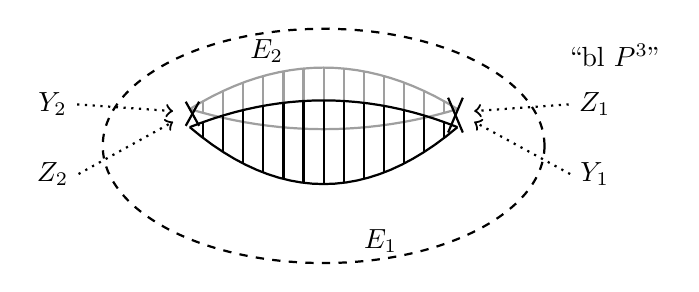
\begin{tikzpicture}[scale=0.85, line width=0.8pt]
  \draw[dashed] (0,0) ellipse (3.3 and 1.75);
  \begin{scope}[gray!75]
    \draw plot[domain=-2.0:2.0] (\x,{0.55+0.62*(1-\x*\x/4)});
    \draw plot[domain=-2.0:2.0] (\x,{0.55-0.30*(1-\x*\x/4)});
    \foreach \x in {-1.8,-1.5,...,1.9}
      \draw (\x,{0.55-0.30*(1-\x*\x/4)}) -- (\x,{0.55+0.62*(1-\x*\x/4)});
  \end{scope}
  \draw plot[domain=-2.0:2.0] (\x,{0.28+0.40*(1-\x*\x/4)});
  \draw plot[domain=-2.0:2.0] (\x,{0.28-0.85*(1-\x*\x/4)});
  \foreach \x in {-1.8,-1.5,...,1.9}
    \draw (\x,{0.28-0.85*(1-\x*\x/4)}) -- (\x,{0.28+0.40*(1-\x*\x/4)});
  \draw (-2.06,0.66) -- (-1.86,0.30);
  \draw (-2.06,0.30) -- (-1.86,0.66);
  \draw (1.86,0.72) -- (2.08,0.20);
  \draw (1.86,0.20) -- (2.08,0.72);
  \node at (-0.85,1.42) {$E_2$};
  \node at (0.85,-1.42) {$E_1$};
  \node (Ytwo) at (-4.05,0.62) {$Y_2$};
  \node (Ztwo) at (-4.05,-0.42) {$Z_2$};
  \node (Zone) at (4.05,0.62) {$Z_1$};
  \node (Yone) at (4.05,-0.42) {$Y_1$};
  \draw[dotted,->] (Ytwo.east) -- (-2.25,0.52);
  \draw[dotted,->] (Ztwo.east) -- (-2.25,0.36);
  \draw[dotted,->] (Zone.west) -- (2.25,0.52);
  \draw[dotted,->] (Yone.west) -- (2.25,0.36);
  \node at (4.35,1.35) {``bl~$\mathbb{P}^3$''};
\end{tikzpicture}
\caption{广中平祐的一个真非\trProjective{}\trSmooth{}三维体之例。（依原书手绘图重绘。）}\label{fig:hironaka-example}
\end{figure}

注意 $\pi$ 是\trProper{}的：它在 $U_1$ 与 $U_2$ 上\trProper，而\trProperness{}这一概念在靶上是局部的（\mbox{命题~11.4.4}(b)）。由于 $\mathbb{P}^3_k$ 是\trProper{}的（在 $k$ 上，\mbox{定理~8.4.10}），而\trProper{}\trMorphism{}的复合仍\trProper（\mbox{命题~11.4.4}(c)），所以 $X$ 是\trProper{}的。

\textbf{24.7.F.（练习）}\quad 证明 $X$ \trSmooth。（提示：\mbox{定理~22.3.10}。）令 $E_i$ 为 $C_i\setminus\{p_1,p_2\}$ 的原像。证明 $\pi|_{E_i}\colon E_i\to C_i\setminus\{p_1,p_2\}$ 是一个 $\mathbb{P}^1$-丛（并且\trFlat）。

\textbf{24.7.G.（练习）}\quad 设 $\overline{E}_i$ 为 $E_i$ 在 $X$ 中的\trClosure。证明 $\overline{E}_i\to C_i$ 是\trFlat{}的。（提示：\mbox{练习~24.3.J}。）

\textbf{24.7.H.（练习）}\quad 证明 $\pi^{-1}(p_i)$ 是两个 $\mathbb{P}^1$ 的并，比如说 $Y_i$ 与 $Z_i$，它们相交于一点，且满足 $Y_i,Y_{3-i},Z_{3-i}\in\overline{E}_i$ 但 $Z_i\notin\overline{E}_i$。

\textbf{24.7.I.（练习）}\quad 按如下思路证明 $X$ 不是\trProjective{}的。假设不然，$\mathscr{L}$ 是 $X$ 上的一个\trVeryAmple{}\trLineBundle，于是 $\mathscr{L}$ 在每条\trCurve{}上都有正的\trDegree（包括诸 $Y_i$ 与 $Z_i$）。利用 $\overline{E}_i\to C_i$ 的\trFlatness{}以及平坦\trFamily{}中\trDegree{}的恒常性（\mbox{练习~24.7.D}），证明 $\deg_{Y_i}\mathscr{L}=\deg_{Y_{3-i}}\mathscr{L}+\deg_{Z_{3-i}}\mathscr{L}$。导出矛盾。（这个论证会让你想起 \S15.2.11 的论证。）

\textbf{24.7.7. 「\trProjective{}\trMorphism」这一概念在靶上不局部。}\quad 注意 $\pi\colon X\to\mathbb{P}^3$ 不是\trProjective{}的，否则 $X$ 就会是\trProjective{}的（因为当最终靶为\trQuasicompact{}时，\trProjective{}\trMorphism{}的复合仍\trProjective，\mbox{练习~17.3.I}）。但在每个 $p_i$ 之外，$\pi$ 都是\trProjective{}的（因为它是诸\trBlowup{}的复合——\trBlowup{}按构造是\trProjective{}的——而最终靶\trQuasicompact，故\mbox{练习~17.3.I} 适用）。于是，「\trProjective{}\trMorphism」这一概念在靶上不局部。（利用 \S15.2.11 可以构造一个更简单但不\trSmooth{}的例子。）
